\documentclass{article}

\usepackage{tikz}

%-----------------------------------------------------------
% Grid

\newlength{\size}
\newcommand{\gogrid}[1][1]{
  \setlength{\size}{\dimexpr #1cm / 18 \relax} % chktex 1

  \draw[step=\size] (0, 0) grid (#1, #1);
  
  \boardoutline{#1}
}

\newcommand{\boardoutline}[1]{
  % Top Horizontal
  \draw[black,line width=1]
    (0, #1) -- (\dimexpr #1cm + 0.01cm, #1); % chktex 1 chktex 8
  % Right Vertical
  \draw[black,line width=1] 
    (#1, 0) -- (#1, #1); % chktex 8
  % Bottom Horizontal
  \draw[black,line width=1]
    (0, 0) -- (\dimexpr #1cm + 0.01cm, 0); % chktex 1 chktex 8
  % Left Vertical
  \draw[black,line width=1]
    (0, 0) -- (0, #1); % chktex 8
}

%-----------------------------------------------------------
% Stones

% \newcommand{stone}[1]{
  
% }

%-----------------------------------------------------------

\begin{document}
  \begin{figure}[ht]
    \begin{center}
      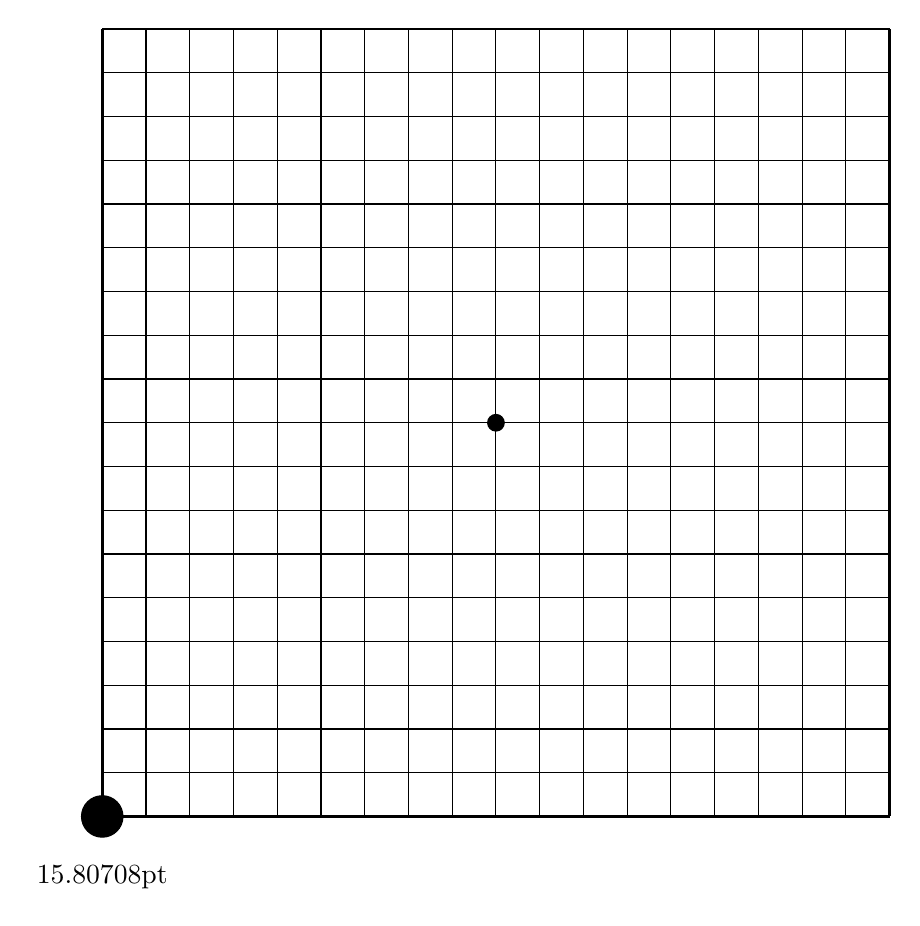
\begin{tikzpicture}
        \gogrid[10]
        \filldraw (0,0) circle [radius=7.48756pt] node[below=0.5cm] {\the\size};
        \filldraw (5,5) circle[radius=3pt];
      \end{tikzpicture}
      \caption{Another grid with two points!}\label{my_grid2}
    \end{center}
  \end{figure}
\end{document}